\chapter{Scelte tecniche ed implementazione}
\label{chap:implementazione}
L'elaborato di tesi sviluppato prevede due progetti distinti. Il primo è il sistema distribuito (abbreviato in SD) ed il secondo progetto si occupa della parte visualizzazione dei risultati che prende il nome di (TORVIAMO UN NOME).
\\ Questo capitolo mette in luce le tecnologie adottate durante la creazione dei due progetti mostrando l'effettiva implementazione.  
\section{Diagramma delle classi}
\label{sec:diagramma delle classi}
\section{Codice}
\label{sec:codice}
L'elaborato di tesi, come detto in precedenza, è suddiviso in due distinti progetti: Sistema Distribuito e Blockchain Explorer. In questo capitolo, l'attenzione sarà focalizzata sulla reale implementazione, visualizzando e commentando righe di codice con maggiore interesse.
\\ Ogni applicazione Java ha un \textit{entry point}, cioè una funzione principale che viene richiamata all'avvio dell'applicativo. All'interno del sistema distribuito l'entry point è definita nella classe \textit{App}. Questa classe ha il compito di:
\begin{itemize}
\item \textbf{Recupero Costanti}: Il primo passo che effettua l'applicazione è il recupero delle costanti definite all'interno di un file di \textit{properties}: \textit{bitcoin.properties}. Per leggere le costanti di questo file utilizza un metodo statico della classe \textit{PropertiesReader} chiamato \textit{readProperties}. Questo metodo [\ref{lst:prop}], prende in input un file di proprieties e restituisce una mappa chiave-valore con tutte le proprietà definite nel file.

\begin{lstlisting}[language=Java, label=lst:prop, caption={Metodo readProperties.}]
public static Map<String, String> readProperties(String propFileName){

	Map<String, String>  propMap = new HashMap<String,String>();
	Properties prop = new Properties();

	try {
	prop.load(PropertiesReader.class.getClassLoader()
	.getResourceAsStream(propFileName));

		for (String key : prop.stringPropertyNames()) {
			String value = prop.getProperty(key);
			propMap.put(key, value);
		}

	} catch (IOException e) {

		e.printStackTrace();

	}

	return propMap;
}
\end{lstlisting}

\item \textbf{Inizializzare Spark e connessione con Bitcoind}: Caricate le costanti in una mappa, non resta che inizializzare Spark. Per fare ciò, viene creato un oggetto di tipo \textit{JavaStreamingContext} [\ref{lst:intiSpark}].

\begin{lstlisting}[language=Java, label=lst:intiSpark, caption={Inizializzazione Spark Streaming.}]
JavaStreamingContext streamingContext = new JavaStreamingContext(sparkConf, new Duration(2000));
\end{lstlisting}

Questa classe si occupa di creare il contesto streaming di Spark secondo le configurazioni presenti nell'oggetto \textit{sparkConf} e di creare Job eseguiti ogni due secondi. All'oggetto \textit{sparkConf} viene dato un nome che lo identifica in caso di più Job,gli viene impostato il tipo di cluster da creare ed infine l'URL di connessione col database Neo4j [\ref{lst:sparkConf}].

\begin{lstlisting}[language=Java, label=lst:sparkConf, caption={Creazione oggetto sparkConf.}]
SparkConf sparkConf = new SparkConf().setAppName(propMap.get("appSparkName"));
					
if (!sparkConf.contains("spark.master")) {
	/*local[K] (Run Spark locally with K threads, 
	usually k is set up to match the number of 
	cores on your machine)*/
	sparkConf.setMaster("local[2]"); 
}

/**
 * Configuration of Neo4j
 * */
sparkConf.set("spark.neo4j.bolt.url", neo4jConnectionUrl);
\end{lstlisting}

Una volta che il contesto di Spark è stato creato, non resta che creare il collegamento tra il Sistema Distribuito e Bitcoind. Questa operazione viene fatta tramite l'utilizzo della libreria \textit{spark-streaming-zeromq} di Apache Bahir. La libreria in questione permette di creare una connessione tra una coda ZMQ (utilizzata da Bitcoind) e Spark [\ref{lst:bahir}].

\begin{lstlisting}[language=Java, label=lst:bahir, caption={Metodo della libreria Spark Streaming ZeroMQ.}]
JavaDStream<byte[]> lines = ZeroMQUtils.createStream(streamingContext, host, subscribe, bytesToObjects );
\end{lstlisting}

Il metodo \textit{createStream} associa, quindi, la ricezione dei dati ad una funzione di callback, che viene richiamata per la gestione dei dati. In questo caso, la funzione in questione è \textit{bytesToObjects} \ref{lst:bytesToObjects}, che estrae i byte provenienti dalla coda di Bitcoind e li trasforma in oggetti parallelizzati: \textit{JavaDStream}.

\begin{lstlisting}[language=Java, label=lst:bytesToObjects, caption={Funzione bytesToObjects.}]
Function<byte[][], Iterable<byte[]>> bytesToObjects = new Function<byte[][], Iterable<byte[]>>() {
            @Override
            public Iterable<byte[]> call(byte[][] bytes) throws Exception {
                Iterable iterable = Arrays.asList(bytes[0]);
                return iterable;
            }
        };
\end{lstlisting}

\item \textbf{Salvare i dati nell'HDFS}: Ottenuti i byte provenienti da Bitcoind può partire l'elaborazione. Il primo step da effettuare è il salvataggio sul filesystem distribuito Hadoop. Questo framework, precedentemente citato, si occupa della storicizzazione distribuita dei dati. Spark, abituato a lavorare su architetture distribuite, ha al suo interno metodi nativi che permettono di salvare dati in Hadoop. Infatti è bastato chiamare il metodo \textit{saveAsTextFile} della classe \textit{RDD} per salvare i dati all'interno del filesystem.

\begin{lstlisting}[language=Java, label=lst:hadoop, caption={Salvataggio Bytes su HDFS.}]
lines.foreachRDD((bytes, time)-> {

	List<byte[]> blockAsByte = bytes.collect();
	if (!blockAsByte.isEmpty()) {
		bytes.coalesce(1).saveAsTextFile(hadoopHdfs + File.separator + "blocks" + File.separator);
	}

});
\end{lstlisting}

Nel listato [\ref{lst:hadoop}] per ogni RDD, viene salvato un file di testo sul filesystem di Hadoop.

\item \textbf{Lanciare il job di Spark}: Terminate le operazioni preliminari, Spark è pronto per eseguire il Job. 
\\Tutti i dati, come visto nel listato \ref{lst:bahir}, sono contenuti in un oggetto chiamato \textit{lines}. Questo oggetto contiene la rappresentazione in byte dei blocchi provenienti da bitcoin, parallelizzati sui vari nodi del cluster. Il primo step da eseguire dunque, è la trasformazione da byte in oggetto.
\begin{itemize}
\item \textbf{Trasformare i Byte in oggetti}: La trasformazione di una sequenza di byte in blocco è demandata a \textit{Bitcoinj}. Questa libreria, creata da Google, è usata per lavorare con il protocollo Bitcoin. Può mantenere un portafoglio, inviare/ricevere transazioni senza bisogno di una copia locale di Bitcoin Core e ha molte altre funzionalità avanzate \cite{bitcoinj:home}. Implementato in Java, offre oggetti e metodi per gestire al meglio i dati provenienti da Bitcoind. 
\\ Nel Job di Spark, quindi, la trasformazione dei byte è fatta dal metodo \textit{blockMakerFromBytes} di \textit{BlockTestNetManager}. Il metodo in questione, partendo da un array di byte restituisce un oggetto che prende il nome di \textit{Block}. Il listato \ref{lst:bitcoindj} mostra la trasformazione dei byte provenienti di Bitcoin ad oggetto Block. 
\begin{lstlisting}[language=Java, label=lst:bitcoindj, caption={Array di Byte trasformato in oggetto Block.}]
BlockTestNetManager blockManager = new BlockTestNetManager();
Block block = blockManager.blockMakerFromBytes(blockAsByte);
\end{lstlisting}
\item \textbf{Salvare in Neo4j}: Per il recupero e l'analisi, le transazioni sono storicizzate nel database a grafi Neo4j. Dall'oggetto \textit{block} precedentemente inizializzato, quindi, vengono recuperate tutte le transazioni tramite il metodo \textit{getTransactions()}. Il metodo restituisce una lista di transazioni (\textit{Transaction}) associate al blocco che il Job salva nel database.
\begin{lstlisting}[language=Java, label=lst:saveNeo, caption={Prelievo transazioni e salvataggio in Neo4j.}]
for (int i = 0; i < block.getTransactions().size(); i++) {
	BitcoinTransaction bTx = new BitcoinTransaction(tx.getHashAsString(),
                                block.getHashAsString(), tx.getInputs(), tx.getOutputs(),
                                i, new Date());
    Transaction tx = block.getTransactions().get(i);
    for(TransactionDBOutput tOut : bTx.getValidReceiver()) {
		log.info("#### Saving transaction in Neo4j ####");
        neo4jManager.createORupdate(Constants.NODE_LABEL, String.join(Constants.STRING_DELIMITER, bTx.getValidSender()), Constants.NODE_LABEL, tOut.getHash(),Constants.RELATIONS_LABEL, Constants.TYPE_OF_MONEY, Double.toString(tOut.getValue()),bTx.getHash() ,bTx.getBlockHash(), df.format(bTx.getReceivedTime()));
	}
}
\end{lstlisting}
Come si vede nel listato \ref{lst:saveNeo}, le transazioni recuperate dal blocco vengono nuovamente trasformate, per comodità, in un oggetto creato ad-hoc \textit{BitcoinTransaction}. Da questo oggetto sono recuperate tutte le transazioni che hanno un valido destinatario (\textit{getValidReceiver()}) e per ognuna di esse viene effettuata una query Cypher \ref{lst:UpdateNeo} che crea o modifica i nodi nel database.

\begin{lstlisting}[language=Java, label=lst:UpdateNeo, caption={Metodo che crea o modifica una transazione in Neo4j.}]
public void createORupdate(String $fromLabel, String $hashFrom, String $toLabel, String $hashTo, String $relationLabel, String $relType, String $relValue, String $transactionHash, String $blockHash, String receivedDate){

	try (Session session = driver.session()) {
		String greeting = session.writeTransaction(new TransactionWork<String>(){

		@Override
		public String execute( Transaction tx ) {
			StatementResult result = 
			
			tx.run("Merge (a:" + $fromLabel + "{hash:'"+ $hashFrom + "'})\n" + "Merge (b:" + $toLabel + "{hash:'" + $hashTo + "'})\n" + "Merge (a)-[r:" + $relationLabel + " {type: '" + $relType + "', value: '" + $relValue + "', transactionHash:'" + $transactionHash +"',blockHash: '" + $blockHash + "', receivedTime:'" + receivedDate + "'}]->(b);", parameters( "","") );
			return "Relationship Saved";
		}

		});
	}
}
\end{lstlisting}
\item \textbf{Calcolo del PageRank}: L'analisi delle transazioni è un'operazione che richiede molta potenza di calcolo. Il sistema distribuito però, tramite il cluster di Spark, riesce a gestire al meglio queste situazioni garantendo alta affidabilità e rapidità d'esecuzione. Nel progetto di tesi, per mostrare la potenza di Spark è stata utilizzato l'algoritmo di PageRank applicato su milioni di nodi.

\begin{lstlisting}[language=Java, label=lst:GraphX, caption={Calcolo PageRank e salvataggio su Neo4j.}]
log.info("### Start PageRank calculation by Graphx ###");

Graph graph = Neo4jGraph.loadGraph(
streamingContext.sparkContext().sc(),
Constants.NODE_LABEL, ScalaUtils.convertListToSeq
(Arrays.asList(Constants.RELATIONS_LABEL)), Constants.NODE_LABEL);

Graph pageRankGraph = PageRank.run(graph,Constants.NUMBER_OF_PAGE_RANK_ITERATIONS,
Constants.RANDOM_RESET_PROBABILITY, 
stringClassTag, stringClassTag);

Neo4jGraph.saveGraph(streamingContext.sparkContext().sc(), pageRankGraph, Constants.NODE_PAGE_RANK_PROP, new Tuple2<String,String>(Constants.RELATIONS_RANK_LABEL, Constants.RELATIONSHIP_PAGE_RANK_PROP) , scala.Option.apply(new Tuple2<String,String>(Constants.NODE_RANK_LABEL, Constants.PAGE_RANK_REFERENCE_ID)), scala.Option.apply(new Tuple2<String,String>(Constants.NODE_RANK_LABEL, Constants.PAGE_RANK_REFERENCE_ID)), true, stringClassTag, stringClassTag);

\end{lstlisting}

Nel codice \ref{lst:GraphX} sono riportare le operazioni che il Job di spark esegue sui nodi esistenti nel sistema. Il primo passo è quello di caricare in una struttura dati tutti i nodi salvati precedentemente. GraphX per questo scopo, mette a disposizione la classe \textit{Graph}.
\\ Caricati i nodi delle transazioni nella struttura dati di Spark viene invocato il metodo \textit{PageRank.run} che esegue il calcolo del PageRank su tutti i nodi del grafo. Questo metodo ritorna un nuovo grafo contenente, per ogni nodo, il valore del PageRank ottenuto.
\\ Terminata l'esecuzione del metodo, non resta che salvare il nuovo grafo ottenuto nella base dati per un impiego futuro.

\item \textbf{Pubblicazione dei dati}: L'ultima operazione del Job è quella di pubblicare i dati per essere fruiti dalle applicazioni in real-time. Il sistema distribuito quindi, riceve da Bitcoin le informazioni, le storicizza, le analizza e le rimette a disposizione per altri consumatori. Le righe di codice  \ref{lst:pubKafka}, mostrano come sono inviati i dati processati, sul topic \textit{transaction-topic} di Kafka. 

\begin{lstlisting}[language=Java, label=lst:pubKafka, caption={Invio dati a Kafka.}]
log.info("#### Sending data to kafka ####");
final Producer<Long, String> producer = KafkaProducerBuilder.createProducer(kafkaHost + ":" + kafkaPort, kafkaAppID );
try {
	log.info("Sending JSON: " + json);
	final ProducerRecord<Long, String> record =
			new ProducerRecord<>(kafkaTopic, new Random().nextLong(),
					json);
	RecordMetadata metadata = producer.send(record).get();
} finally {
	producer.flush();
	producer.close();
}
\end{lstlisting}

In particolare, in queste poche righe di codice, viene creato un oggetto KafkaProducer, il quale ha il compito di connettersi al \textit{kafkaHost} e di inviare, tramite il metodo \textit{send}, i dati sul topic settato nel \textit{ProducerRecord}. 

\end{itemize}
\end{itemize} 

Per visualizzare le elaborazioni del sistema distribuito, è stata creata una applicazione web. Blockchain Explorer infatti, è un sito web che mette a disposizione strumenti per controllare le ultime transazioni, i risultati dell'analisi e la navigazione dell'intera Blockchain. Il codice di questo applicativo può essere riassunto tramite una serie di funzioni:

\begin{itemize}
\item \textbf{Creazione del server}: NodeJs per servire le varie richieste, provenienti dai client, ha bisogno di creare un server. Il modulo che permette questa funzionalità è \textit{http}. Per questo elaborato però, il server è demandato alla libreria Express.js che ci facilita l'implementazione.

\begin{lstlisting}[language=Javascript, label=lst:serverNode, caption={Creazione server in NodeJS.}]
const app = express();
const port = process.env.PORT || 3000;

app.listen(port, function () {
    console.log('express-handlebars example server listening on: ' + port);
});
\end{lstlisting}
Il listato \ref{lst:serverNode} mostra come sia possibile creare un server in NodeJS. Nello specifico, viene creata una variabile chiamata \textit{app}, inizializzata ad \textit{express}, che contiene l'intero web server. L'applicazione con queste poche righe di codice è in grado di rispondere a migliaia di richieste HTTP da parte dei client.

\item \textbf{Associazione URL-Callback}: Ogni richiesta effettuata da i client ad uno specifico endpoint (URL), nel server, è associata ad una funzione di callback. La funzione dunque viene eseguita ogni qualvolta un utente richiede una specifica pagina. L'associazione URL-Callback è gestita tramite il modulo Express.js.

\begin{lstlisting}[language=Javascript, label=lst:express, caption={Associazione URL-Callback in Express.}]
app.get('/infotransaction', function (req, res, next ) {

    var transactionID = req.query.id || '';

    if(transactionID != ''){

        findTransaction(res, req, next, transactionID);

    } else {

        return next('No transaction id');

    }

});
\end{lstlisting}
Nel listato \ref{lst:express}, è possibile notare l'associazione tra l'URL \textit{infotransaction} e la funzione anonima descritta dopo la virgola. Lo scopo di questo URL è quello di ottenere informazioni di una precisa transazione, noto l'ID, all'interno della base dati. Il compito della funzione dunque, è quello di cercare la transazione e di ritornare una pagina HTML con le informazioni richieste. Se la ricerca non dovesse ottenere un risultato, allora la funzione chiama il metodo \textit{next}, il quale permette ad Express.js di eseguire la prossima funzione nella catena di funzioni. In questo caso, viene passata all'handler che si occupa di generare un errore. L'immagine  \ref{fig:transactionDetail} mostra la pagina web che l'utente visualizza, quando richiede il dettaglio di una transazione.  

\begin{figure}[H]
	\centering
	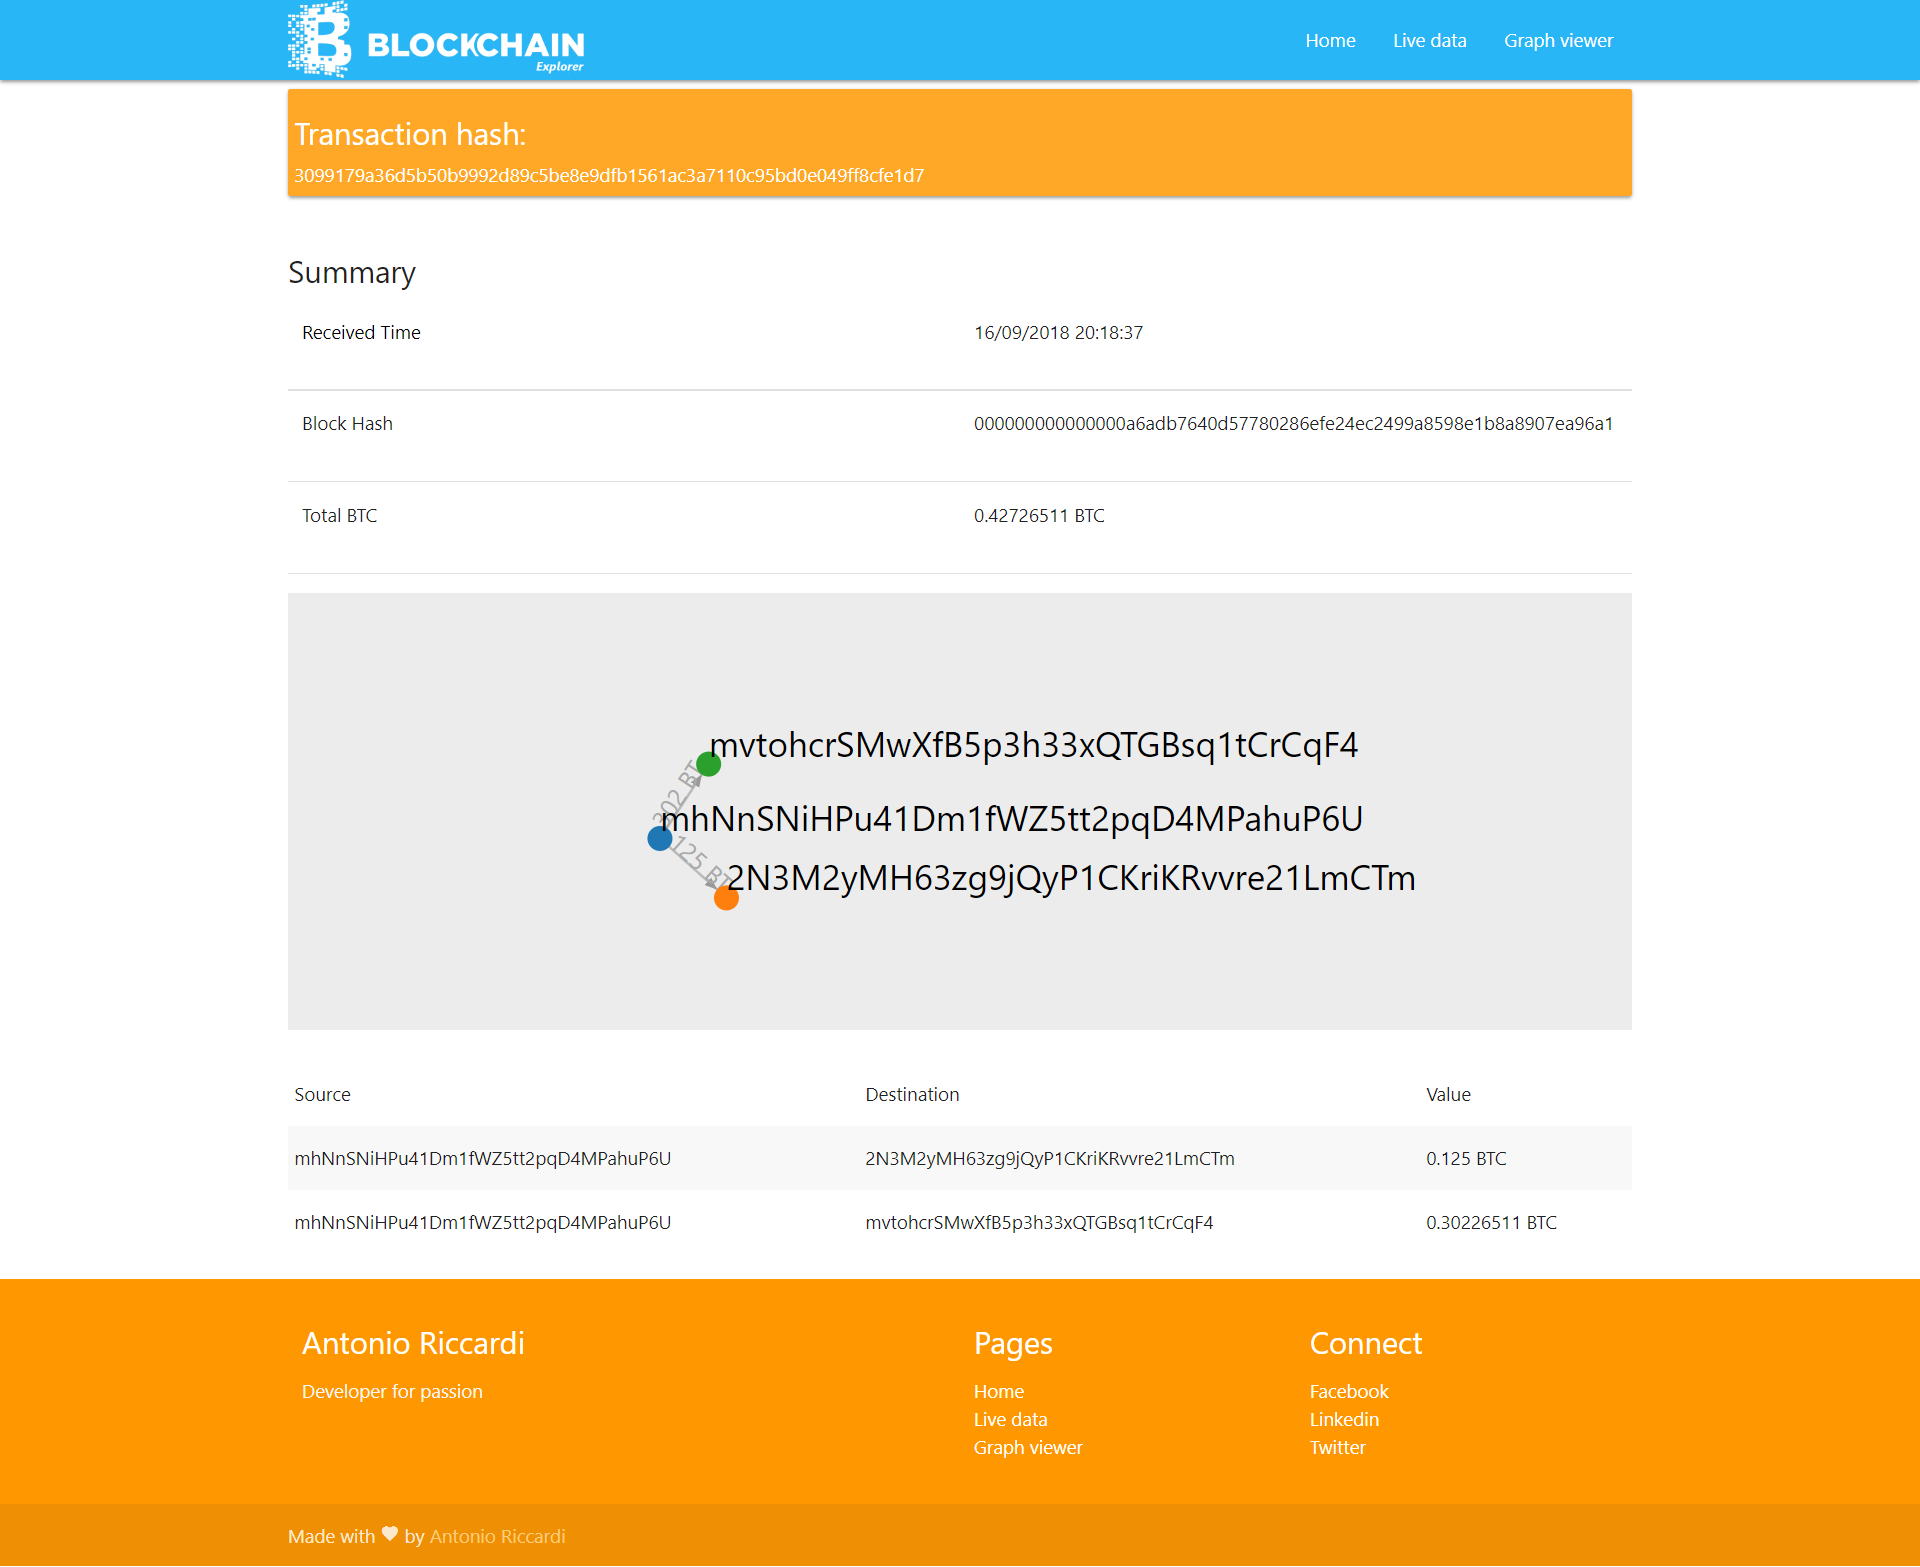
\includegraphics[width=\textwidth]{images/infoTransaction2.png}
	\caption{Dettaglio transazione.}
	\label{fig:transactionDetail}
\end{figure}
 
\item \textbf{Prelievo dati da Kafka}: Come detto in precedenza, il sistema distribuito al termine della propria elaborazione, pubblica i dati sui topic di Kafka. Blockchain Explorer, preleva i dati messi a disposizione dal topic di Kafka implementando un \textit{HighLevelConsumer}. L'oggetto in questione infatti si connette a Kafka e preleva i dati dal topic \textit{transaction-topic}. Infine li invia tramite websocket ai client che sono in ascolto sul server.
\begin{lstlisting}[language=Javascript, label=lst:kafka, caption={Creazione subscriber Kafka.}]

const kafkaBroker = config.kafka.host + ":" + config.kafka.port;
const client = new kafka.Client(kafkaBroker);
const topics = [
    {
        topic: config.kafka.topic
    }
];
const options = {
    autoCommit: true,
    encoding: 'utf8',
    groupId: 'bitcoin-webapp' //Math.random().toString()
};

const consumer = new kafka.HighLevelConsumer(client, topics, options);

consumer.on('message', function(message){
    console.log('Incoming message: ' + message.value.toString());
    wss.sendBrodcast(message.value.toString());
});
\end{lstlisting}

Il codice \ref{lst:kafka} mostra come la WebApp crea un HighLevelConsumer. Nello specifico viene creato un client, \textit{kafka.Client}, contenente l'IP e la porta di Kafka. Inoltre viene creato un oggetto \textit{topic} nella quale viene specificato il topic alla quale connettersi. I due oggetti, insieme ad altre opzioni \textit{options}, sono passate al costruttore dell'oggetto HighLevelConsumer il quale instaura una connessione con la coda e preleva i dati.
\\Infine, all'oggetto \textit{consumer} viene associata una funzione da eseguire ogni qualvolta un nuovo dato è disponibile. Questa funzione ha il compito di inviare i dati, tramite WebSocket, a tutti i client connessi al server.

\item \textbf{Comunicazione tramite Websocket}: Per permettere la comunicazione real-time delle transazioni provenienti da Kafka ai vari client, la WebApp crea un  server WebSocket. La creazione del server è visibile nel listato \ref{lst:websocket}.

\begin{lstlisting}[language=Javascript, label=lst:websocket, caption={Creazione di un Server WebSocket.}]
var wss = new webSocket.Server({
    port: config.webSocket.port
});


wss.sendBrodcast = function(message){
  wss.clients.forEach( function (client) {
     client.send(message);
  });
};
\end{lstlisting}

Infine, al Server WebSocket viene aggiunta la funzione \textit{sendBrodcast}, richiamata nel listato di Kafka \ref{lst:kafka}, la quale ha il compito di inviare a tutti i client connessi al server il messaggio, \textit{message}, proveniente da Kafka.
\item \textbf{Renderizzazione dei Grafi}: La renderizzazione dei grafi è demandata ai browser dei client. Il codice che segue viene inglobato nelle pagine HTML inviate dal server ai vari client. Il browser quindi, riceve dal server sia i dati che il codice da eseguire, generando una pagina come in figura \ref{fig:graphView}.

\begin{lstlisting}[language=Javascript, label=lst:intGraph, caption={Inizializzazione svg per il grafo.}]
var svg = d3.select("#" + idSvg),
        width = + $("#" + idSvg).width(),
        height = +svg.attr("height");

    var zoomLayer = svg.append('g');

    svg.call(d3.zoom().on('zoom', function(){
        zoomLayer.attr('transform', d3.event.transform);
    }));

    zoomLayer.append('defs').append('marker')
        .attrs({'id':'arrowhead',
            'viewBox':'-0 -5 10 10',
            'refX':13,
            'refY':0,
            'orient':'auto',
            'markerWidth':13,
            'markerHeight':13,
            'xoverflow':'visible'})
        .append('svg:path')
        .attr('d', 'M 0,-5 L 10 ,0 L 0,5')
        .attr('fill', '#999')
        .style('stroke','none');
\end{lstlisting}

Nel listato \ref{lst:intGraph} sono riportate le righe di codice che servono per l'inizializzazione del tag \textit{svg}, presente nella pagina HTML, nella quale verranno disegnate cerchi e le linee rappresentati rispettivamente nodi ed archi del grafo delle transazioni di bitcoin. Inoltre, su di esso viene aggiunto un layer per lo zoom, che permette all'utente finale di avere una fluida navigazione all'interno del grafo.

\begin{figure}[H]
	\centering
	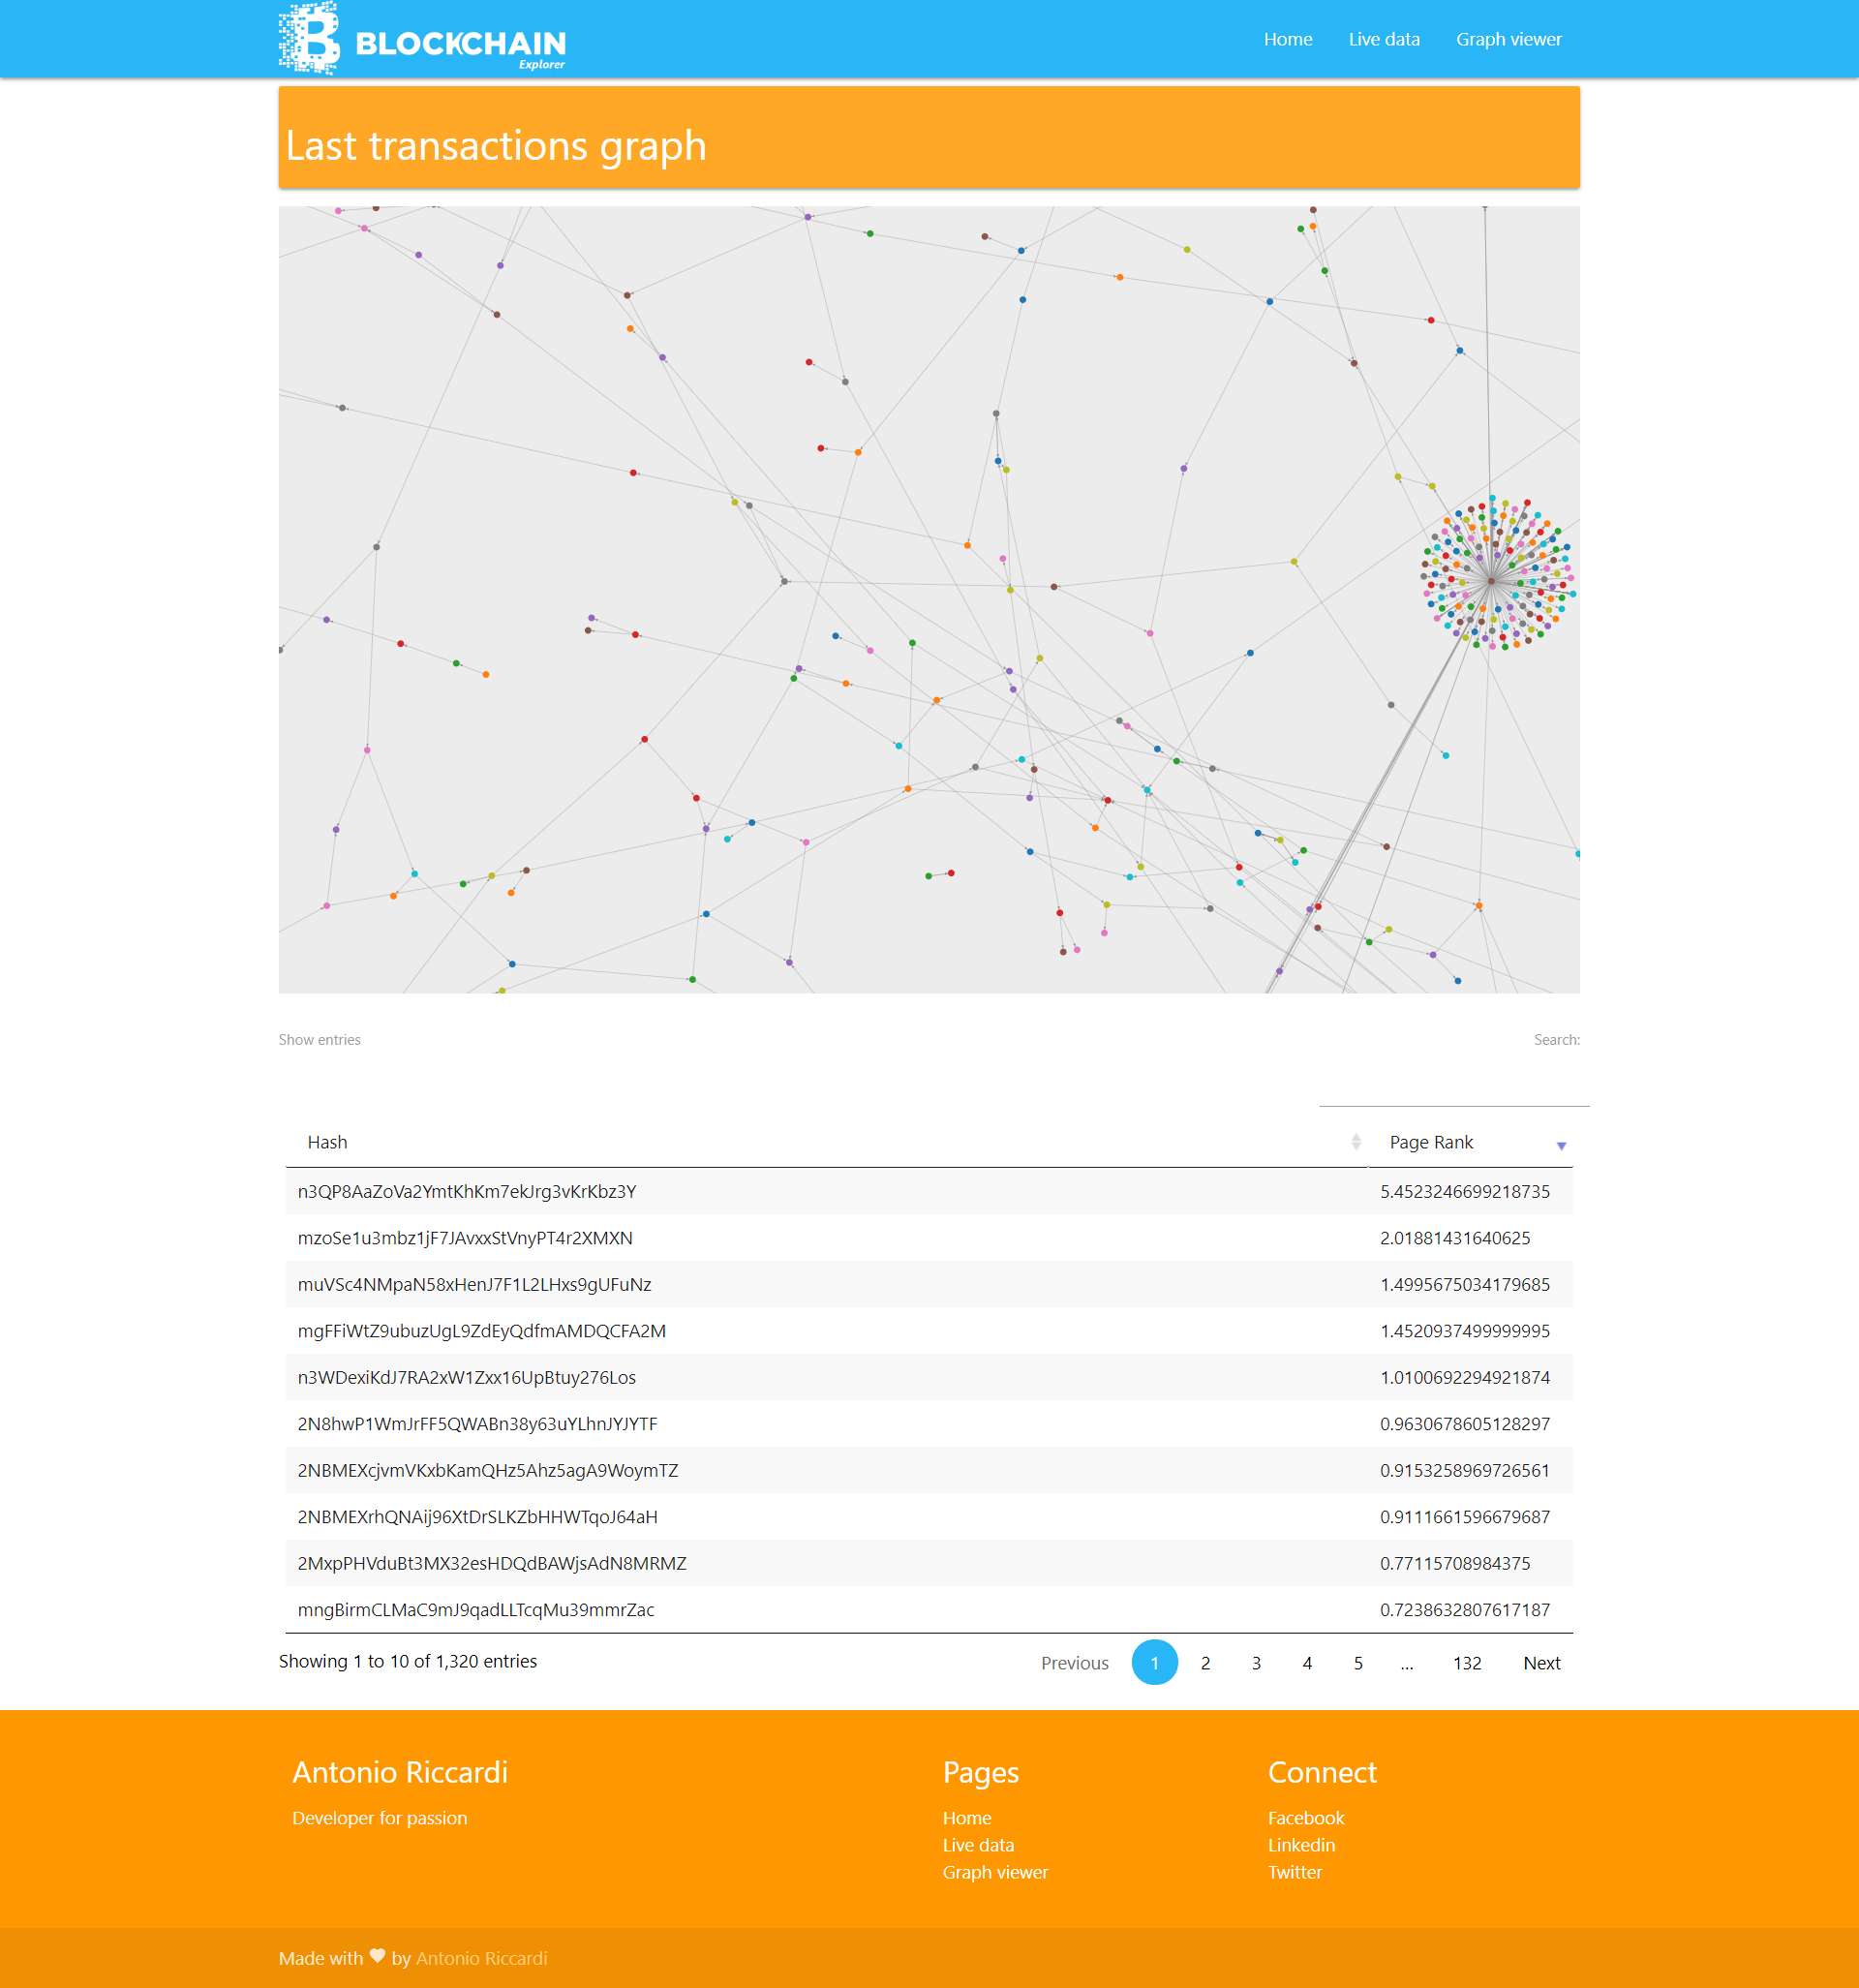
\includegraphics[width=\textwidth, height=0.50\textheight]{images/graphView.png}
	\caption{Grafo delle transazioni completo.}
	\label{fig:graphView}
\end{figure}


\begin{lstlisting}[language=Javascript, escapechar=|, label=lst:drawLine, caption={Creazione linee.}]
		simulation = d3.forceSimulation(nodes)
                            .force("link", d3.forceLink()
                            .id(function (d) { return d.hash;}))
                            .force("charge", d3.forceManyBody().strength(-80))
                            .force("center", d3.forceCenter(width / 2, height / 2))
                            .on("tick", tick)
                            .stop();

        simulation.force("link")|\label{line:link}|
            .links(links);

        for(i=0; i < 300; i++) simulation.tick();


        link.append("title")
            .text(function (d) {
                var t = "Transaction Hash: " + d.transactionHash + "\n" +
                        "Received Time: " + d.receivedTime + "\n" +
                        "Block Hash: " + d.blockHash + "\n" +
                        "Value: " + d.value;
                return t;

            });
\end{lstlisting}


Mentre, nel listato \ref{lst:drawLine} sono riportate le righe di codice utili alla creazione degli archi tra i vari nodi del grafo. In particolare, alla riga \ref{line:link} viene utilizzato il metodo \textit{link} di d3.js che prende in input i dati da renderizzare, i quali sono trasformati in elementi grafici dell'svg chiamati \textit{line}. A questi sono aggiunti le coordinate di partenza e destinazione, l'icona a forma di freccia e l'attributo \textit{title} contenente tutte le informazioni relative alla transazione (Hash, Timestam, valore totale della transazione e l'hash del blocco di appartenenza ).

\begin{lstlisting}[language=Javascript, escapechar=|, label=lst:drawNode, caption={Creazione dei nodi del grafo.}]

        node = zoomLayer
            .selectAll(".node")
            .data(nodes) |\label{line:nodes}|
            .enter()
            .append("g")
            .attr("class", "node")
            .attr("transform", function(d){ 
            return "translate(" + d.x + ", " + d.y + ")";})
            .on("contextmenu", function(data,index){
                console.info("Selected hash: " + data.hash);
                $("input[type='search']").val(data.hash);
                $("input[type='search']").keyup();
                d3.event.preventDefault();

            })
            .call(d3.drag()
                .on("start", dragstarted)
                .on("drag", dragged)
                .on("end", dragended)
            );

        node.append("circle")
            .attr("r", 5)
            .style("fill", function (d, i) {return colors(i);})


        node.append("title")
            .text(function (d) {return d.hash;});
\end{lstlisting}

Analogamente a quanto fatto per gli archi del grafo, nel listato \ref{lst:drawNode} viene mostrato come con D3.js sia possibile associare i dati esistenti in memoria ad elementi grafici sullo schermo. In questo caso, viene utilizzato il metodo \textit{data}, riga \ref{line:nodes}, per passare i nodi da disegnare nella pagina HTML al framework. I nodi, quindi, vengono disegnati tramite il tag \textit{circle} e correlati dalla classe \textit{node} che darà un colore diverso per ogni nodo. Infine, come accade agli archi, viene aggiunto un \textit{title} il quale contiene l'hash dei destinatari o mittenti delle transazioni.
 
\item \textbf{Costruzione delle tabelle}: Altro aspetto importante è la creazione delle tabelle. In Blockchain explorer è possibile visionare in forma tabellare le ultime transazioni processate, la sintesi di una transazione singola oppure i valori del PageRank per ogni hash. Nel codice \ref{lst:table}  è possibile vedere come sia facile trasformare una semplice \textit{<table>} HTML in una tabella con colonne ordinabili, paginazione e filtri di ricerca. Il tutto viene fatto dalla funzione \textit{DataTable(dataTableConfig)} il quale invoca la libreria DataTable che trasforma la tabella \textit{realTimeTransactions} con le proprietà inserite nella variabile \textit{dataTableConfig}.

\begin{lstlisting}[language=Javascript, label=lst:table, caption={Utilizzo DataTable.}]
var initializeTable = function(){
    transactionsTable = $('#realTimeTransactions').DataTable(dataTableConfig);
}

var dataTableConfig = {
    retrieve: true,
    data: [],
    dom: 'ftrip',
    order: [[2, 'desc']],
    columns:[
        {title: 'Transaction hash', className: '', orderable: false, visible: true},
        {title: 'Value Out', className: '', orderable: false, visible: true},
        {title: '', className: '', orderable: true, visible: false},
        {title: '', className: '', orderable: false, visible: false}
    ],
    oLanguage: {
        sEmptyTable: 'Waiting for transactions...'
    }
};
\end{lstlisting}

\item \textbf{HTML Templating}: Come detto in precedenza il server invia pagine HTML dinamiche partendo da template statici. Questa funzionalità è espletata da Express.js. In particolare la libreria permette di utilizzare un motore grafico per renderizzare le pagine HTML. Nell'elaborato di tesi viene utilizzato Handlebars. Il codice \ref{lst:render} mostra come sia semplice associare questo tool come motore grafico di Express. L'associazione viene fatta tramite il metodo \textit{engine}, il quale prende in ingresso una serie di informazioni quali: il template di default, le cartelle contenenti i template ed i partials ed una lista di funzioni, chiamate \textit{helpers}, che possono essere richiamate all'interno dell'HTML. 

\begin{lstlisting}[language=Javascript, label=lst:render, caption={Associazione Express-Handelbars.}]
// Create `ExpressHandlebars` instance with a default layout.
var hbs = exphbs.create({
    defaultLayout: 'main',
    layoutsDir: 'src/views/layouts/',
    partialsDir: 'src/views/partials/',
    helpers: {
        json : function(content) {
            return JSON.stringify(content);
        }
    }
});
app.engine('handlebars', hbs.engine);
\end{lstlisting}

Un template quindi non è altro che una pagina statica HTML, la quale in fase di run-time viene processata e modificata in base alle informazioni provenienti dal server. Un esempio di template è il listato \ref{lst:handleb}, il quale mostra la creazione dinamica delle righe della tabella, partendo dall'oggetto \textit{transaction} ricevuto dal server. Come si può notare, viene usato il costrutto \textit{each} per iterare sull'intero oggetto transaction e di prelevare solo le proprietà da inserire all'interno dei vari \textit{<td>}.

\begin{lstlisting}[language=Javascript, label=lst:handleb, caption={Template Handlebars.}]
<div class="row">
    <table class="table striped">

        <thead>
            <tr>
                <td>Source</td>
                <td>Destination</td>
                <td>Value</td>
            </tr>
        </thead>
        <tbody>
            {{#each transaction}}
                <tr>
                    <td>{{source.properties.hash}}</td>
                    <td>{{destination.properties.hash}}</td>
                    <td>{{relation.properties.value}} BTC</td>
                </tr>
            {{/each}}
        </tbody>
    </table>
</div>
\end{lstlisting}

%TODO Metti figura lista di transazioni

\begin{figure}[H]
	\centering
	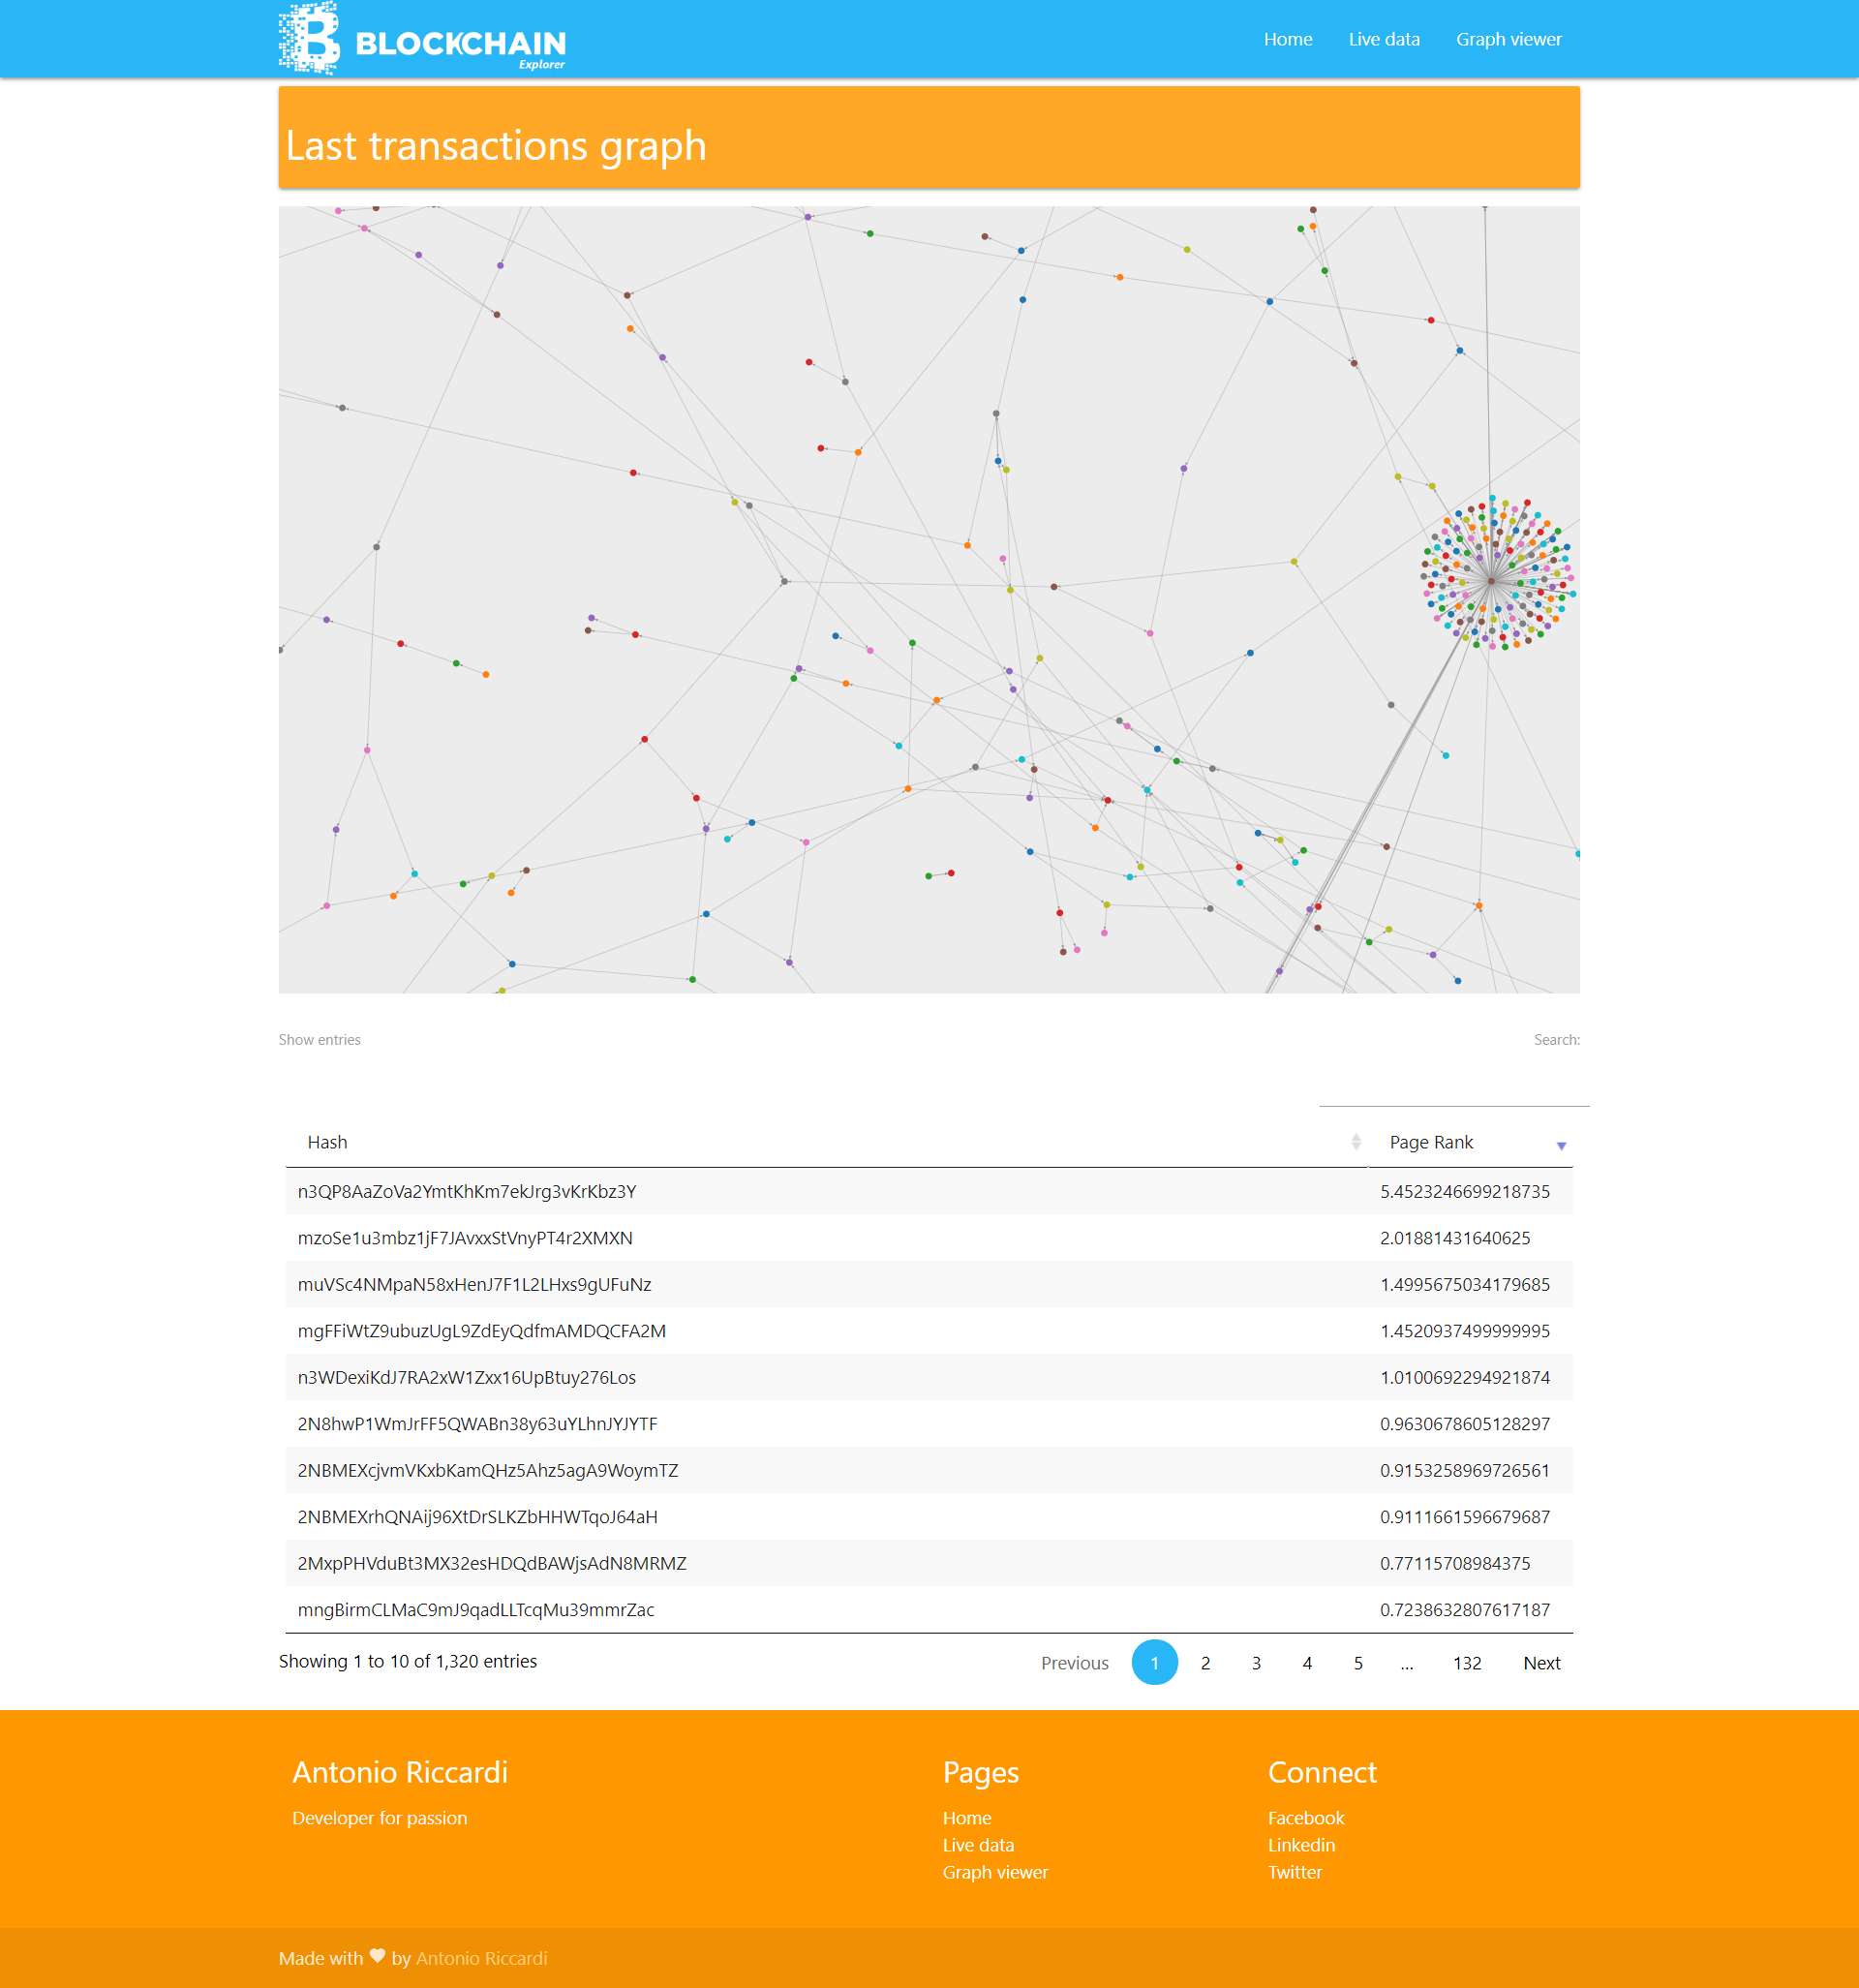
\includegraphics[width=\textwidth, height=0.80\textheight]{images/graphView.png}
	\caption{Grafo delle transazioni completo.}
	\label{fig:tableView}
\end{figure}

In figura \ref{fig:tableView} è possibile visualizzare la pagina HTML che viene generata dall'elaborazione del codice \ref{lst:handleb}. 

\end{itemize}
\section{GitHub}
\label{sec:github}
GitHub è un servizio di hosting per progetti software. Il nome "GitHub" deriva dal fatto che GitHub è una implementazione dello strumento di controllo versione distribuito \textit{Git} \cite{git:wiki}, inventato da Linus Torvalds anima e per anni programmatore di Linux. 
\\ GIT quindi è un version control system (VCS), e cioè un programma che permette di tener traccia di tutte le modifiche e le evoluzione effettuate nel corso della stesura di un codice o di un qualsiasi progetto su supporto digitale.
\\ Un software VCS permette di mantenere una copia del proprio codice
sorgente, sia in locale sia in remoto, senza incorrere in un eccessivo dispendio di energie e senza deconcentrarsi eccessivamente dalla stesure del proprio testo. In linea di principio un VCS permette di tenere sotto controllo qualsiasi documento, siano essi foto, documenti realizzati con programma di videoscrittura, fogli di calcolo, ecc.
\\ Git è diverso dai sistemi di controllo delle versioni precedenti come \textit{Subversion} in quanto è distribuito piuttosto che centralizzato. La differenza maggiore tra i due sistemi è la posizione del codice (repository): 
\begin{itemize}
\item \textbf{Centralizzato}: Tutto il software viene inviato dai programmatori direttamente ad un server centrale che detiene il repository.
\item \textbf{Distribuito}: Non esiste un server centrale, ma esistono repository locali (la macchina di sviluppo) e repository remoti (GitHub).
\end{itemize}
Per questo motivo, GIT è abbastanza veloce, soprattutto dal momento che la maggior parte delle operazioni avviene sul repository locale. Tuttavia, l'utilizzo di Git aggiunge un livello di complessità. L'invio di codice al repository locale e l'invio di commit a un repository remoto sono passaggi separati.
\\ GitHub dunque viene usato come repository remoto di Git da migliaia di sviluppatori poiché gratuito. Inoltre fornisce strumenti utili come il \textit{bug traking}, tool per controllare le differenze tra i file, possibilità di visualizzare cronologia dei commit ed una sezione per commenti ed suggerimenti.
\\ Per l'elaborato di tesi è stato usato questo sistema per tenere traccia delle modifiche apportate al codice. Questo ha permesso in molti casi di ripristinare una versione funzionante del software dopo l'immissione di nuove modifiche. GitHub inoltre, è stato utilizzato per permettere a chiunque volesse riprendere il progetto, modificarlo o applicare delle correzioni, semplicemente \textit{clonando} il repository.
\\I due elaborati di tesi possono essere clonati ai seguenti URL:
\begin{itemize}
\item \textbf{Sistema Distribuito}: \href{https://github.com/Antonio90/BitcoinSpark.git}{https://github.com/Antonio90/BitcoinSpark.git}.
\item \textbf{Blockchain Explorer}: \href{https://github.com/Antonio90/bitcoin-webapp.git}{https://github.com/Antonio90/bitcoin-webapp.git}. 
\end{itemize}